% $Id: comp.tex 8643 2009-07-14 12:25:48Z alexandra $
% Local Variables:
% ispell-check-comments: nil
% Local IspellDict: american
% End:
% --------------------------------------------------------
% User documentation
% copyright by BREDEX GmbH 2005
% --------------------------------------------------------
\label{overviewabstcomp}
The following diagram shows which abstract components \app{} uses and for which actions they can be used for.  


\begin{figure}
\begin{center}
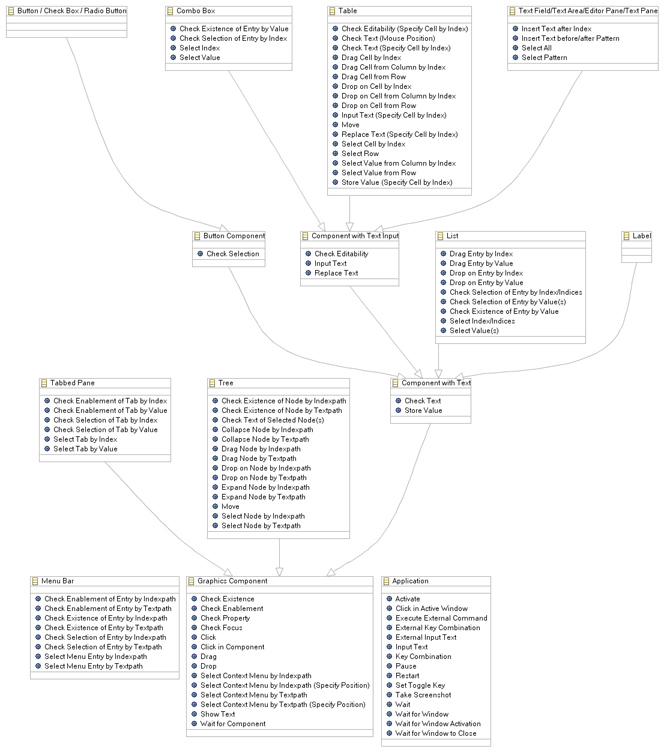
\includegraphics[width=15cm]{Overview/PS/GUIdancerComponentHierarchysmall}
\caption{\app{} component structure}
\label{comp}
\end{center}
\end{figure}

Figure \ref{comp} provides an overview of \app{}'s concrete and abstract component structure. This figure can be interpreted as follows: the arrows show inheritance relations between the components. Thus, a \bxname{Label} component has no actions of its own, but inherits them all from \bxname{Component with Text}. The \bxname{Label} component also inherits any actions that \bxname{Component with Text} also inherited. In this case, these are the actions from \bxname{Graphics component}. 

\clearpage
